\documentclass{article}

\usepackage[utf8]{inputenc}
\usepackage[T1]{fontenc}
\usepackage[greek,english]{babel}
\usepackage{alphabeta}
\usepackage{amsmath}
\usepackage{amssymb}
\usepackage{graphicx}
\usepackage{subcaption}
\usepackage{epstopdf}
\usepackage[margin=1in, paperwidth=8.3in,paperheight=11.7in]{geometry}
\usepackage{hyperref}
\usepackage{paracol}

\newcommand\course{ΗΡΥ 411}
\newcommand\courseName{Ενσωματωμένα Συστήματα Μικροεπεξεργατών}
\newcommand\semester{Χειμερινό 2020-2021}
\newcommand\assignmentNumber{Εργαστήριο 9}
\newcommand\studentName{Μαυρογιώργης Δημήτρης}                           
\newcommand\studentNumber{2016030016}

\title{\underline{\textbf{\assignmentNumber}}} 
\author{\textsc{\textbf{Όνομα:}}  \studentName\\
		\textsc{\textbf{ΑΜ:}}  \studentNumber\\
		\course \ - \courseName\\ 
		\textsc{Πολυτεχνείο Κρήτης}
		}
\date{\today}
\begin{document}
	\maketitle

\section*{Σκοπός}
	Σκοπός του έβδομου και ένατου εργαστηρίου είναι να γράψουμε κώδικα που να αφαιρεί την αναπήδηση από έναν διακόπτη SPDT με δύο διαφορετικούς τρόπους: α) με δειγματοληψία της εισόδου αρκετά συχνά, δηλαδή με polling βασισμένο στον TIMER0, καθώς και β) με εξωτερικά interrupts

\section*{Debouncing Χωρίς Interrupts – με Polling βασισμένο στον TIMER0}
	Aρχικά, δηλώθηκαν κάποια macro, για να ελέγχουμε αν καποιο bit είναι set ή clear, να θέτουμε κάποιο bit σε "0" ή "1" και για εναλλαγή κάποιου bit από "0" σε "1" και το αντίστροφο. Στο main πρόγραμμα αρχικοποιούμε τον TIMER0, ενεργοποιούμε τα interrupt και τέλος έχουμε ένα while loop στο οποίο δεν κάνουμε τίποτα, καθώς όλα θα γίνονται στον handler του TIMER0.\\
	
	\begin{figure}[h!]
		\centering
		\begin{subfigure}[t]{0.5\textwidth}
			\centering
			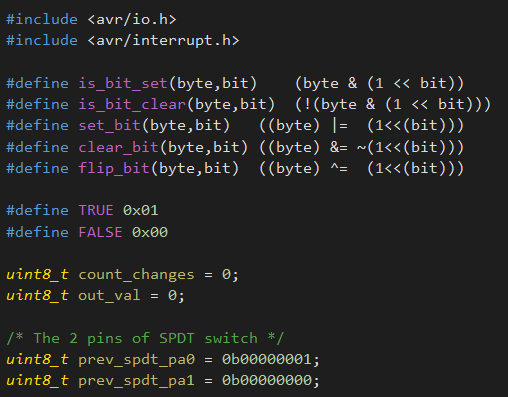
\includegraphics[height=4cm, width=\linewidth]{./results/lab9_defines_a.png}
			\caption{C code for defines}
		\end{subfigure}%
		~
		\begin{subfigure}[t]{0.5\textwidth}
			\centering
			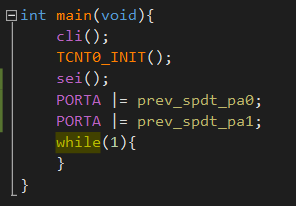
\includegraphics[height=4cm, width=\linewidth]{./results/lab9_main_a.png}
			\caption{C code for main}
		\end{subfigure}
	\end{figure}
	
	\noindent
	Για το σκοπό της συγκεκριμένης υλοποίησης χρησιμοποιήθηκε ο TIMER0 του 1 ms από τα προηγούμενα εργαστήρια. Στο service routine του TIMER0 κάνουμε τη δειγματοληψία της εισόδου κάθε 1 ms και κάθε φορά αποθηκεύουμε τις τιμές έτσι, ώστε να τις συγκρίνουμε με τις επόμενης περιόδου. Επιπλέον, εκτός από την αποθήκευση, ελέγχουμε τις προηγούμενες τιμές με τις τωρινές και ποιο bit άλλαξε από την προηγούμενη περίοδο, για να δούμε ποιος ακροδέκτης του SPDT έχει τις αναπηδήσεις, και αναλόγως θέτουμε τη έξοδο 0 ή 1. \\
	
	\noindent
	Ειδικότερα, αν άλλαξε το bit PA1, ελέγχουμε ποια ήταν η προηγούμενη τιμή του. Αν άλλαξε από "1" σε "0". Τότε θερωρούμε ότι σε αυτό τον κύκλο έκανε bounce η είσοδος PA1 και θέτουμε το bit PA2 στο "0". Στην αντίστροφη, περίπτωση διατηρούμε την έξοδο "1". Αν τώρα έχουμε και στις δύο εισόδους "1", απλά αποθηκεύουμε ως έξοδο την προηγούμενη τιμή. Τέλος, η κατάσταση "0" και στους δύο ακροδέκτες δεν είναι δυνατή, γιατί δεν γίνεται να είναι ενεργοποιημένοι και οι δύο ακροδέκτες του SPDT ταυτόχρονα. Ομοίως με τα παραπάνω γίνονται οι ίδιο έλεγχοι για το αν άλλαξε το PA0 τιμή από την προηγούμενη δειγματοληψία. \\
	
	\noindent
	Τέλος, αν δεν άλλαξε κάποιος ακροδέκτης τιμή, απλώς αυξάνουμε την τιμή ενός counter και μόλις η τιμή του φτάσει το 0x0A, δηλαδή έχουν περάσει 10 ms, βγάζουμε την έξοδο.
	
	\pagebreak
	\begin{figure}[h!]
		\centering
		\begin{subfigure}[t]{0.5\textwidth}
			\centering
			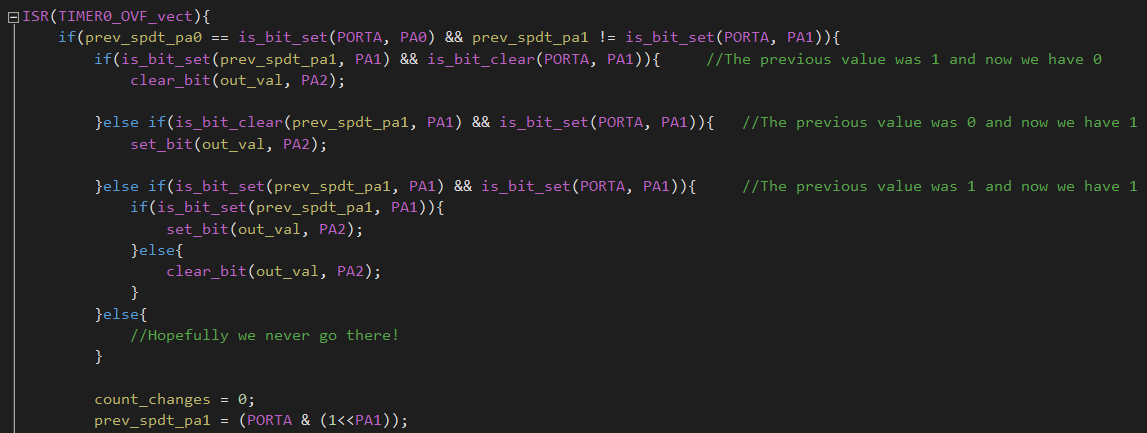
\includegraphics[height=3cm, width=\linewidth]{./results/lab9_timer0_a_a.png}
		\end{subfigure}%
		~
		\begin{subfigure}[t]{0.5\textwidth}
			\centering
			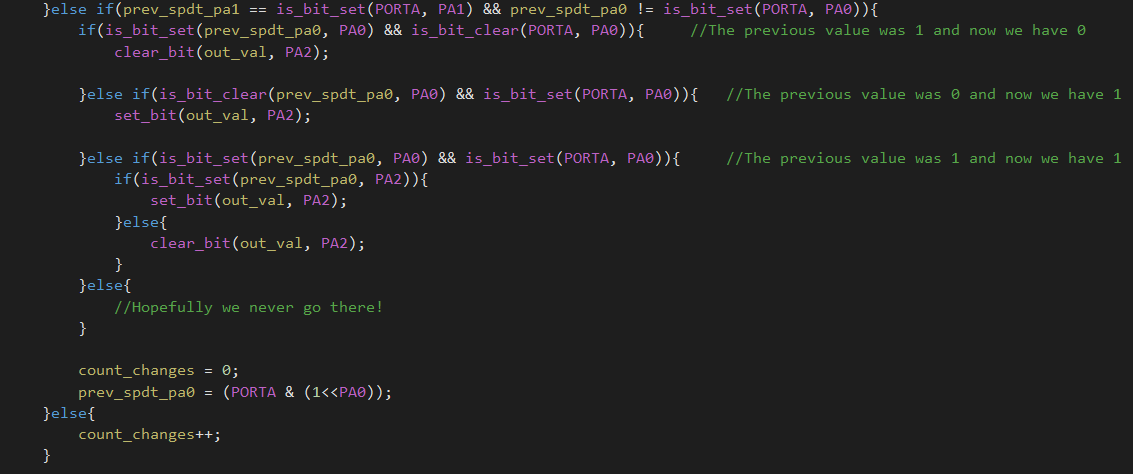
\includegraphics[height=3cm, width=\linewidth]{./results/lab9_timer0_b_a.png}
		\end{subfigure}
		
		\begin{subfigure}[t]{0.5\textwidth}
			\centering
			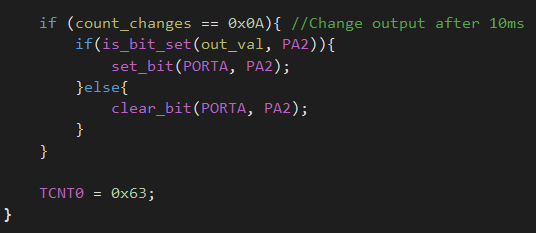
\includegraphics[height=3cm, width=\linewidth]{./results/lab9_timer0_c_a.png}
		\end{subfigure}
		\caption{C code for TIMER0 inerrupt handler}
	\end{figure}

	\noindent
	\textbf{Προσομοίωση Αποτελεσμάτων} \\
	\noindent
	Αρχικά, προσομοιώνουμε τα bounches και από 1-1 που είναι οι δύο είσοδοι, γίνονται 1-0 και στη συνέχεια ξανά 1-1. Όπως φαίνεται στις δύο πρώτες εικόνες, η έξοδος από "0" γίνεται "1", αφού κατασταλάξει η έξοδος και περάσουν τα 10 ms. Ομοίως, στις επόμενες δύο εικόνες, η προσομοίωση γίνεται με περισσότερα bounches από την αρχική και βλέπουμε ότι η έξοδος από "1" που ήταν, άλλαξε σε "0" μετά από επίσης 10 ms και αφού σταμάτησαν τα bounches.
	
	\begin{figure}[h!]
		\centering
		\begin{subfigure}[t]{0.5\textwidth}
			\centering
			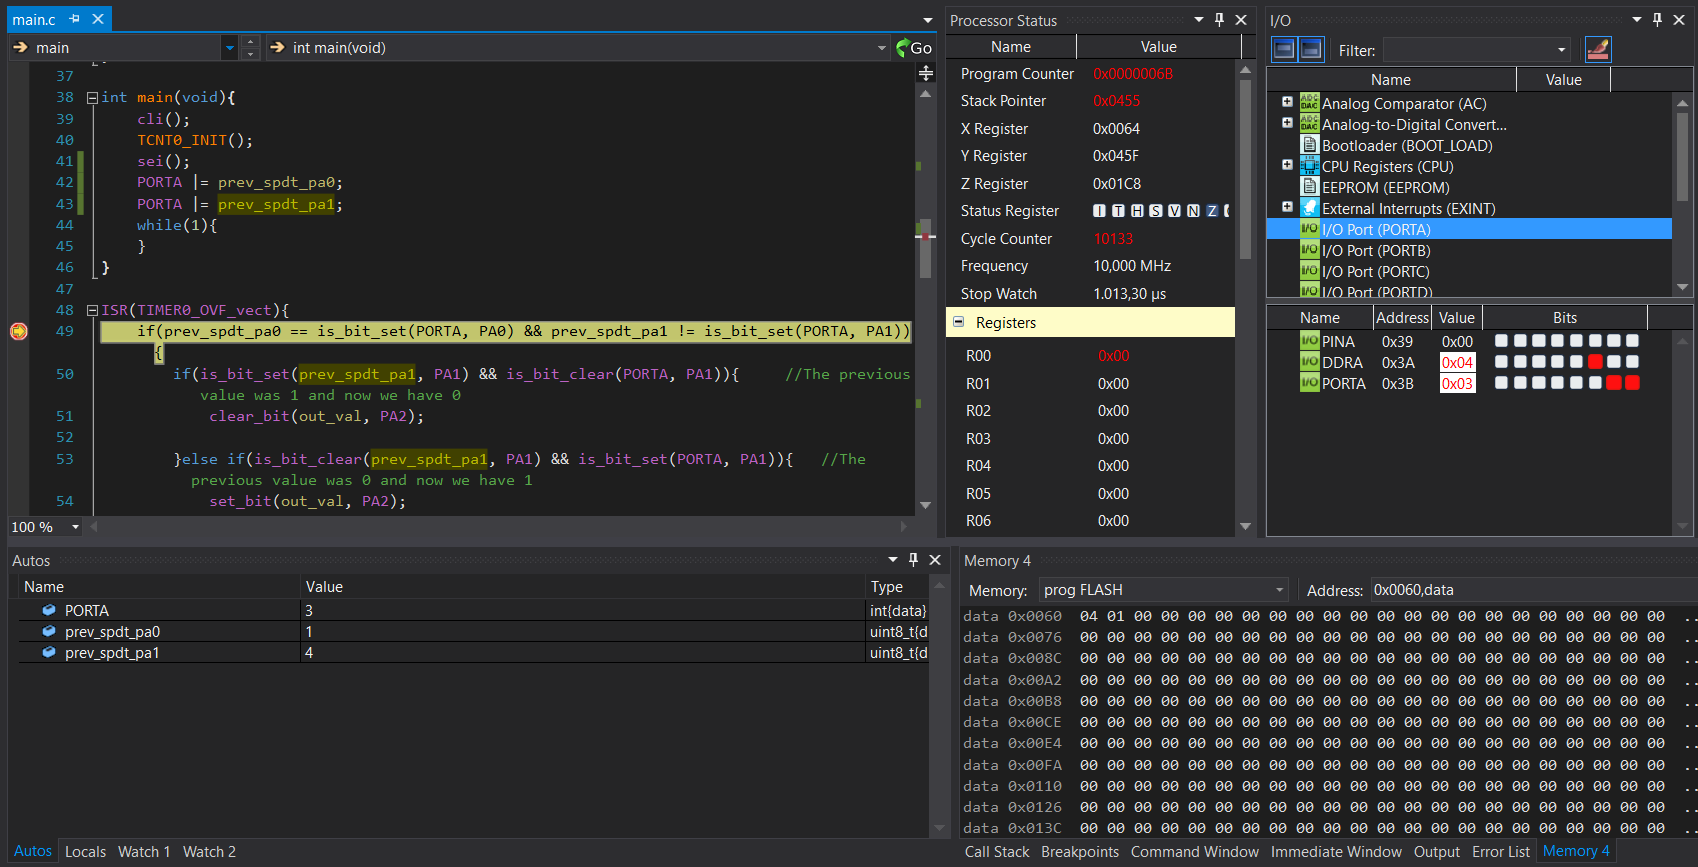
\includegraphics[height=3cm, width=\linewidth]{./results/lab9_sim_a_a.png}
		\end{subfigure}%
		~
		\begin{subfigure}[t]{0.5\textwidth}
			\centering
			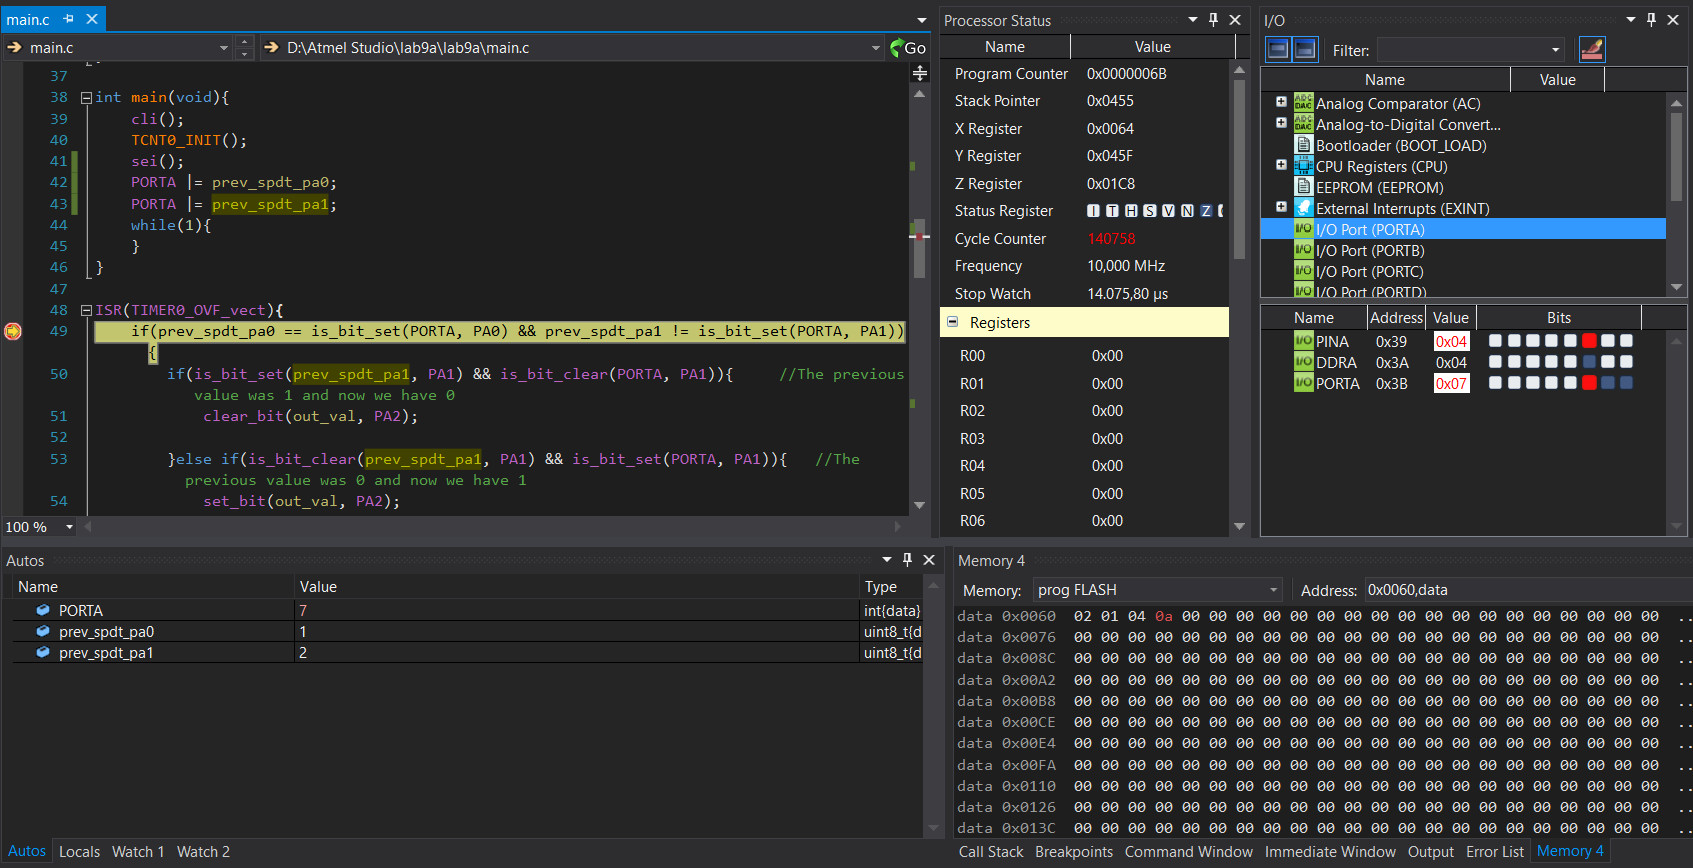
\includegraphics[height=3cm, width=\linewidth]{./results/lab9_sim_b_a.png}
		\end{subfigure}
		\caption{Results from Αtmel Studio 7 - Change from "0" to "1"}
		
		\begin{subfigure}[t]{0.5\textwidth}
			\centering
			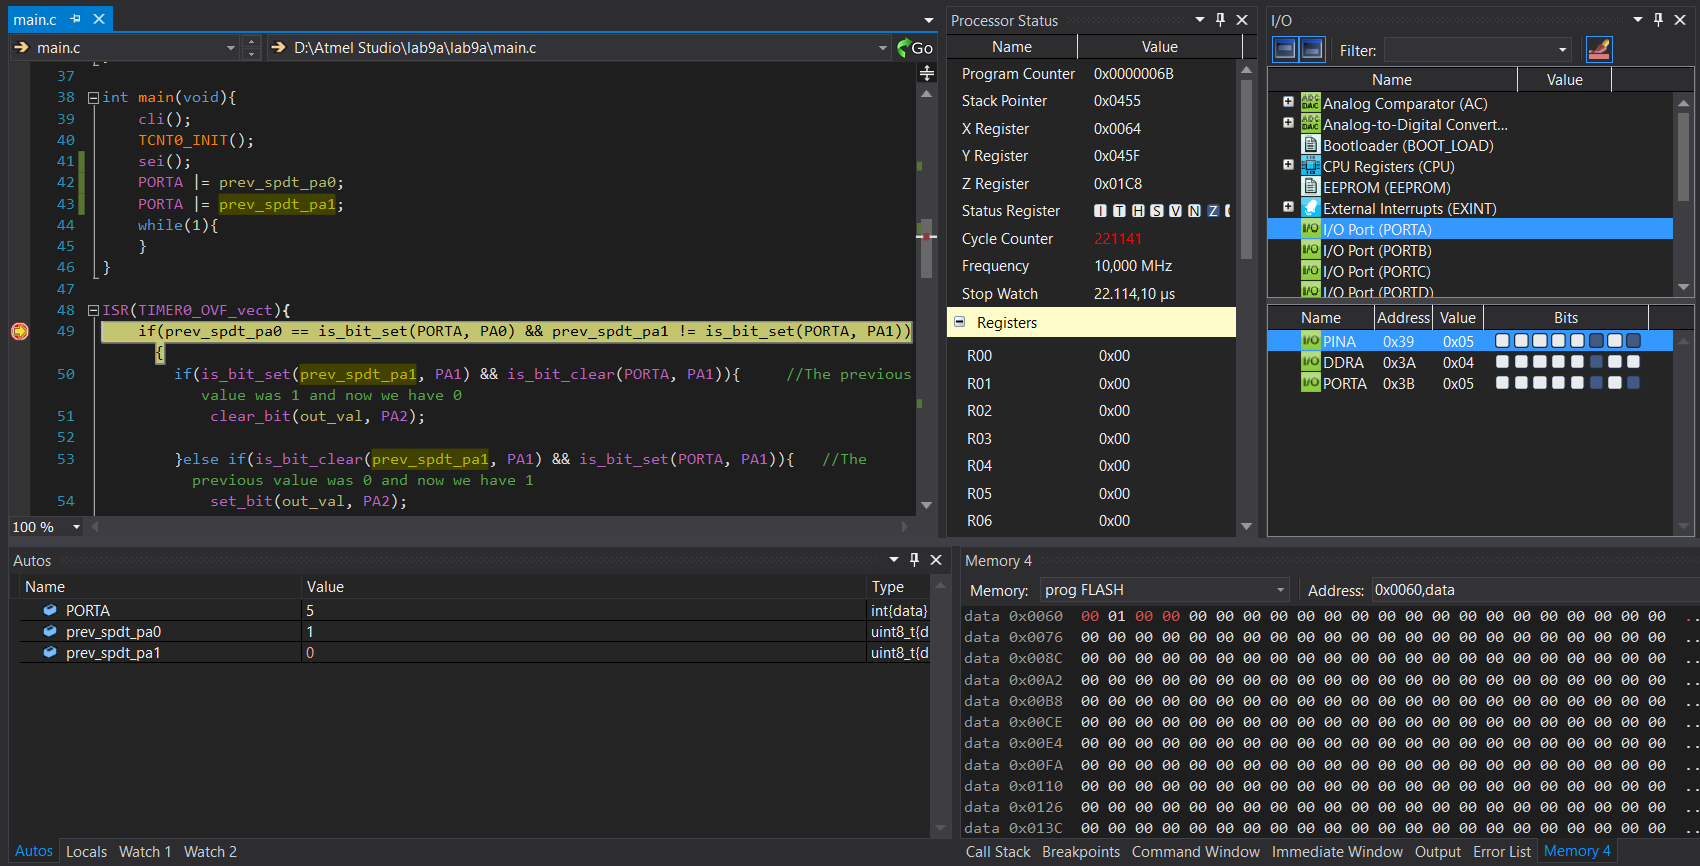
\includegraphics[height=3cm, width=\linewidth]{./results/lab9_sim_c_a.png}
		\end{subfigure}%
		~
		\begin{subfigure}[t]{0.5\textwidth}
			\centering
			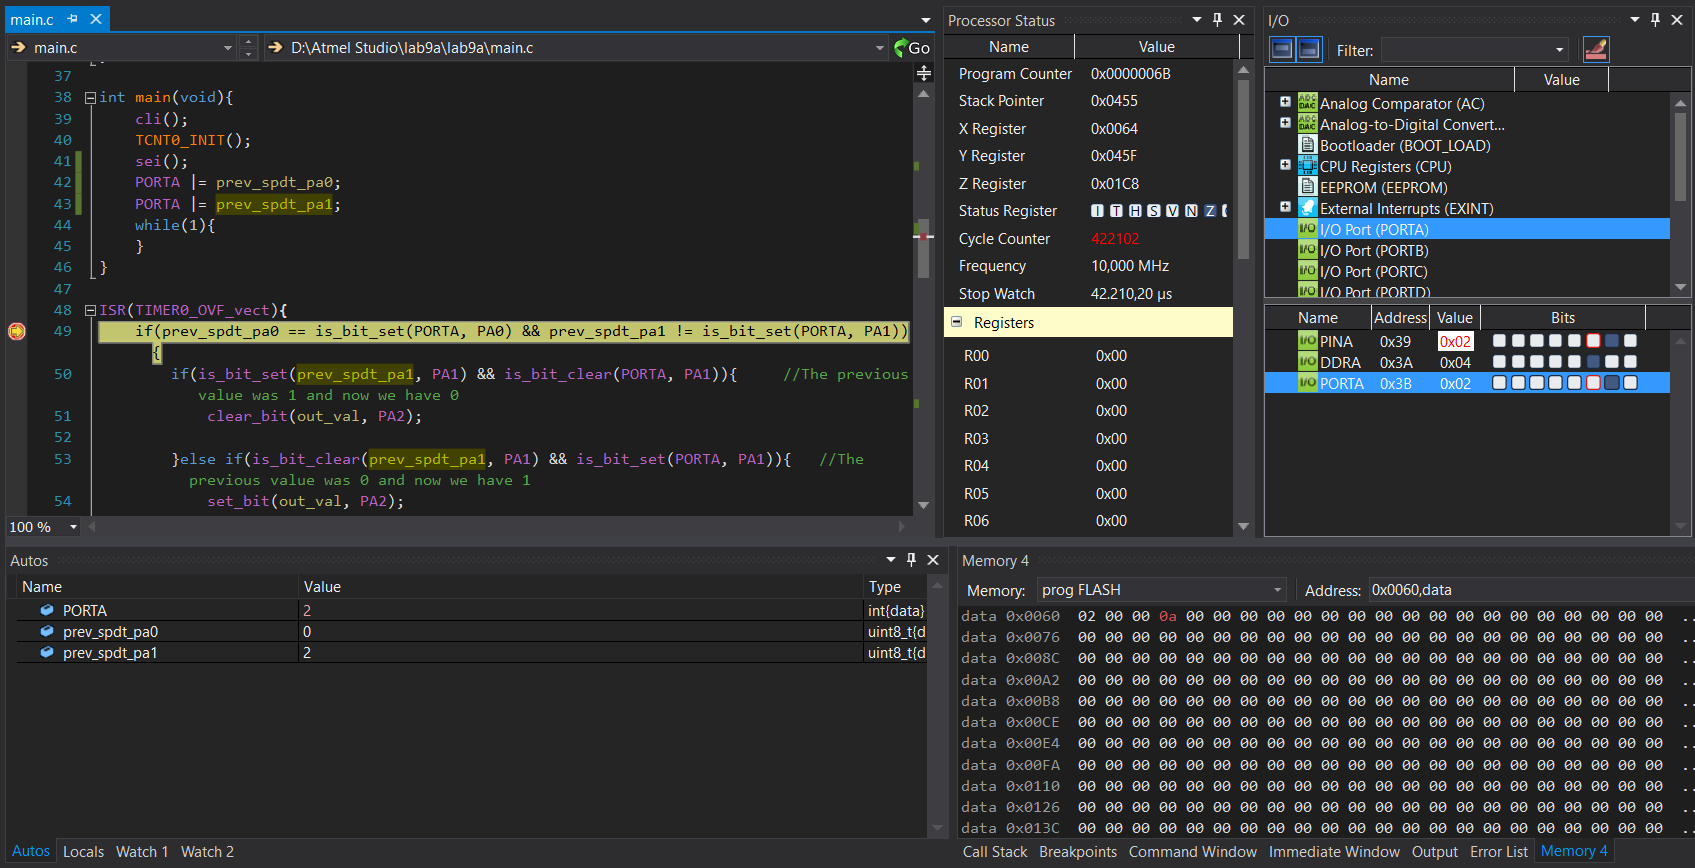
\includegraphics[height=3cm, width=\linewidth]{./results/lab9_sim_d_a.png}
		\end{subfigure}
	    \caption{Results from Αtmel Studio 7 - Change from "1" to "0"}
	\end{figure}
\pagebreak
\section*{Debouncing με Interrupts}
	Ομοίως με την περίπτωση χωρίς external interrupt, δηλώθηκαν κάποια macro, για να ελέγχουμε αν καποιο bit είναι set ή clear, να θέτουμε κάποιο bit σε "0" ή "1" και για εναλλαγή κάποιου bit από "0" σε "1" και το αντίστροφο. Επιπλέον, για τη χρήση external interrupt ενεργοποιούμε τα bit INT0 και INT1 στον καταχωρητή GICR, ενώ για την ανίχνευση των αναπηδήσεων, χρειαζόμαστε να ανιχνεύουμε falling edges. Γι' αυτό θέτουμε σε "1" τα bit ISC11 και ISC01. 
	\begin{figure}[h!]
		\centering
		\begin{subfigure}[t]{0.5\textwidth}
			\centering
			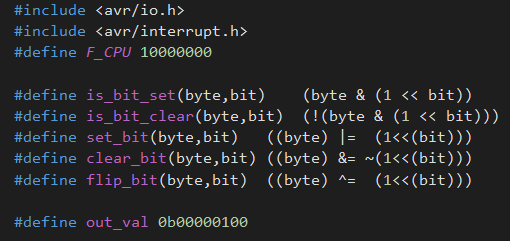
\includegraphics[height=4cm, width=\linewidth]{./results/lab9_defines_b.png}
			\caption{C code for defines}
		\end{subfigure}%
		~
		\begin{subfigure}[t]{0.5\textwidth}
			\centering
			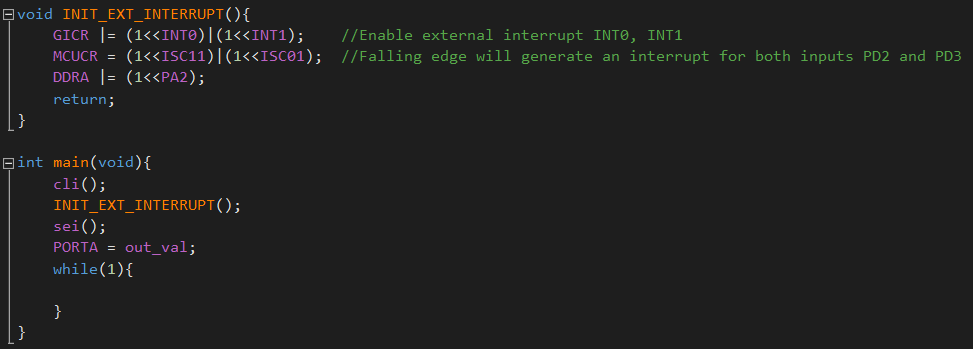
\includegraphics[height=4cm, width=\linewidth]{./results/lab9_main_b.png}
			\caption{C code for main}
		\end{subfigure}
	\end{figure}
	
	\noindent
	Για την αλλαγή ανίχνευση των αναπηδήσεων, ελέγχουμε μόλις έρθει κάποιο falling edge την τιμή της άλλης εισόδου, πχ για το INT0, το οποίο εκτελείται όταν βρεθέι κάποιο falling edge στο PD2 έχουμε δύο περιπτώσεις: Αν το PD3 ήταν "1" τότε σημαίνει ότι τα bounches βρίσκονται στο PD2. Οπότε κάνουμε την έξοδο "0". Αν τώρα το PD3 είναι "0" σε κάποιο falling edge, σημαίνει ότι στο PD2 υπήρξε μια αυξομείωση τάσης και σε αυτό το σενάριο διατηρούμε "1" την έξοδο. Ομοίως, και στον δεύτερο handler ελέγχουμε για τις ίδιες περιπτώσεις με μοναδική διαφορά ότι σε αυτή την περίπτωση αν το PD2 είναι "1" και έχουμε falling edge στο PD3, τότε διατηρούμε την έξοδο "1", αλλιώς την κάνουμε "0". 
	\begin{figure}[h!]
		\centering
		\begin{subfigure}[t]{0.5\textwidth}
			\centering
			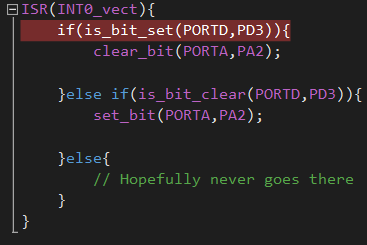
\includegraphics[height=4cm, width=\linewidth]{./results/lab9_int0_b.png}
		\end{subfigure}%
		~
		\begin{subfigure}[t]{0.5\textwidth}
			\centering
			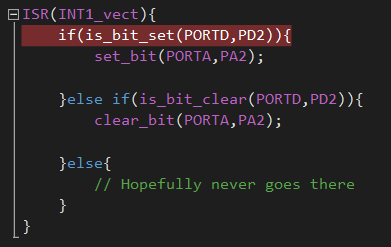
\includegraphics[height=4cm, width=\linewidth]{./results/lab9_int1_b.png}
		\end{subfigure}
		\caption{C code for the two external interrupt handlers}
	\end{figure}
	
	\noindent
	\textbf{Προσομοίωση Αποτελεσμάτων} \\
	\noindent
	
	\noindent
	Σε αυτή την περίπτωση βλέπουμε ότι με το που ανιχνευτεί κάποιο falling edge εκτελείται ο αντίστοιχος handler και ελέγχει σε ποια περίπτωση βρισκόμαστε από αυτες που αναλύθηκαν παραπάνω. Στις πρώτες δύο εικόνες, βλέπουμε ότι η έξοδος από "1" άλλαξε σε "0" μετά από περίπου 25000 κύκλους, όπως συμβαίνει και στο stimuli file όπου για 25000 η έξοδος είναι "1" και έπειτα αλλάζει σε "0". Ομοίως, στις επόμενες δύο εικόνες βλέπουμε ότι εκτελείται ο δεύτερος handler και η έξοδος αλλάζει από "0" σε "1".	Επομένως, βλέπουμε ότι με αυτό τον τρόπο η ανίχνευση των bounches είναι γρηγορότερη σε σχέση με τη μεθοδο του polling και TIMER0, καθώς με το που βρεθέι κάποιο falling edge που σημαίνει κατ' επέκταση αλλαγή κάποιας εισόδου, μπορούμε να αλλάξουμε απευθείας την έξοδο ανάλογα με τις τιμές που έχουν αυτές οι είσοδοι. 
	\pagebreak
	\begin{figure}[h!]
		\centering
		\begin{subfigure}[t]{0.5\textwidth}
			\centering
			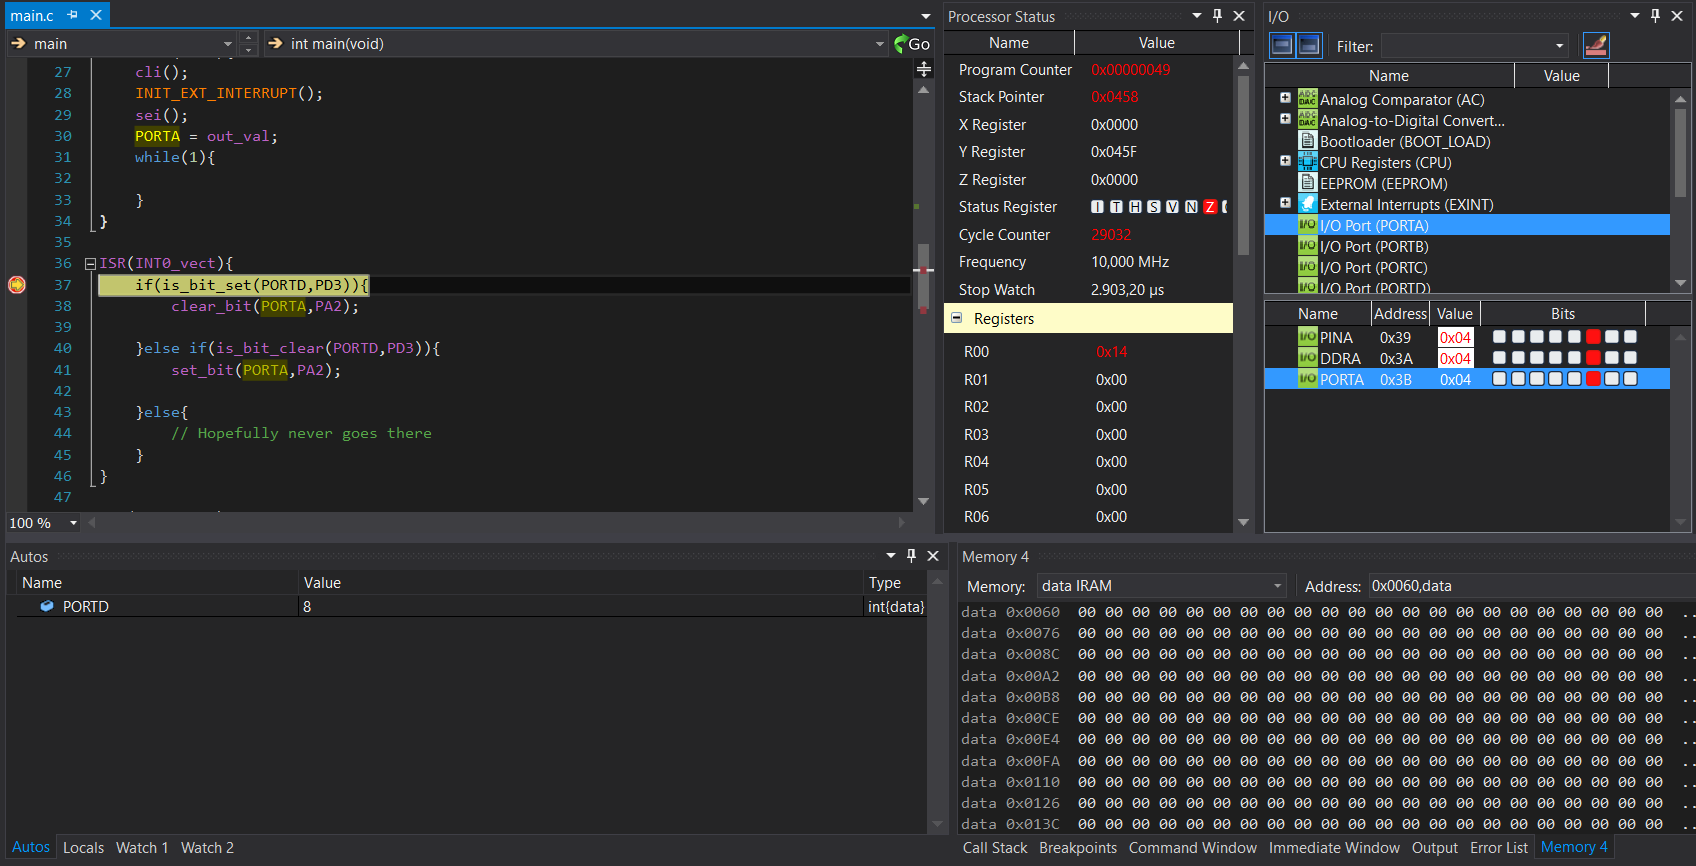
\includegraphics[height=3cm, width=\linewidth]{./results/lab9_sim_a_b.png}
		\end{subfigure}%
		~
		\begin{subfigure}[t]{0.5\textwidth}
			\centering
			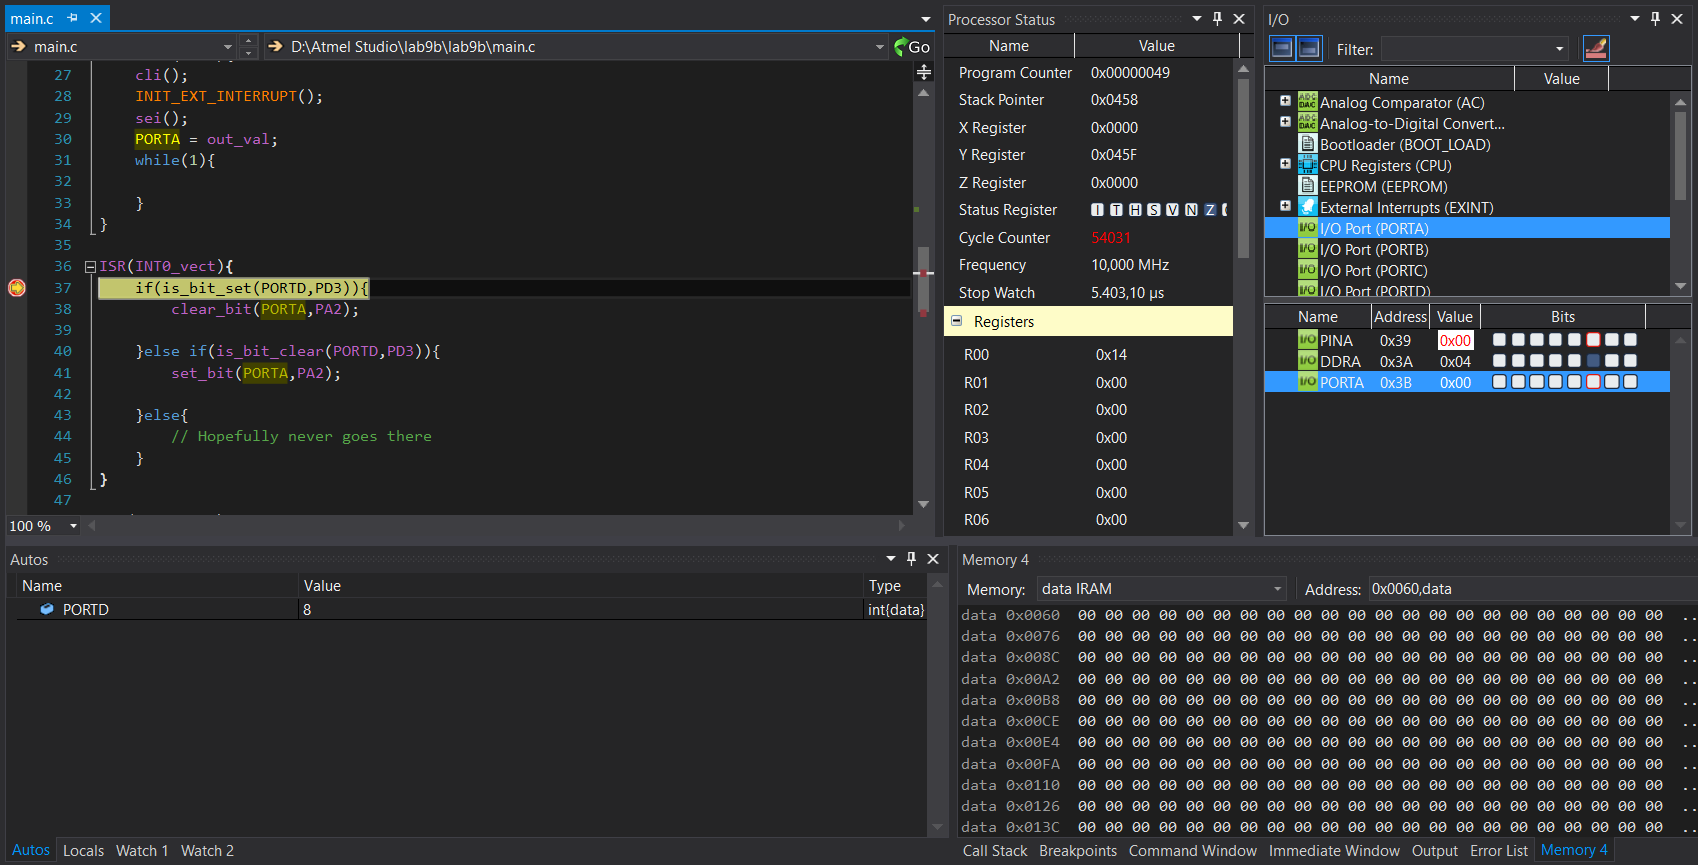
\includegraphics[height=3cm, width=\linewidth]{./results/lab9_sim_b_b.png}
		\end{subfigure}
		\caption{Results from Αtmel Studio 7 - Change from "0" to "1"}
		
		\begin{subfigure}[t]{0.5\textwidth}
			\centering
			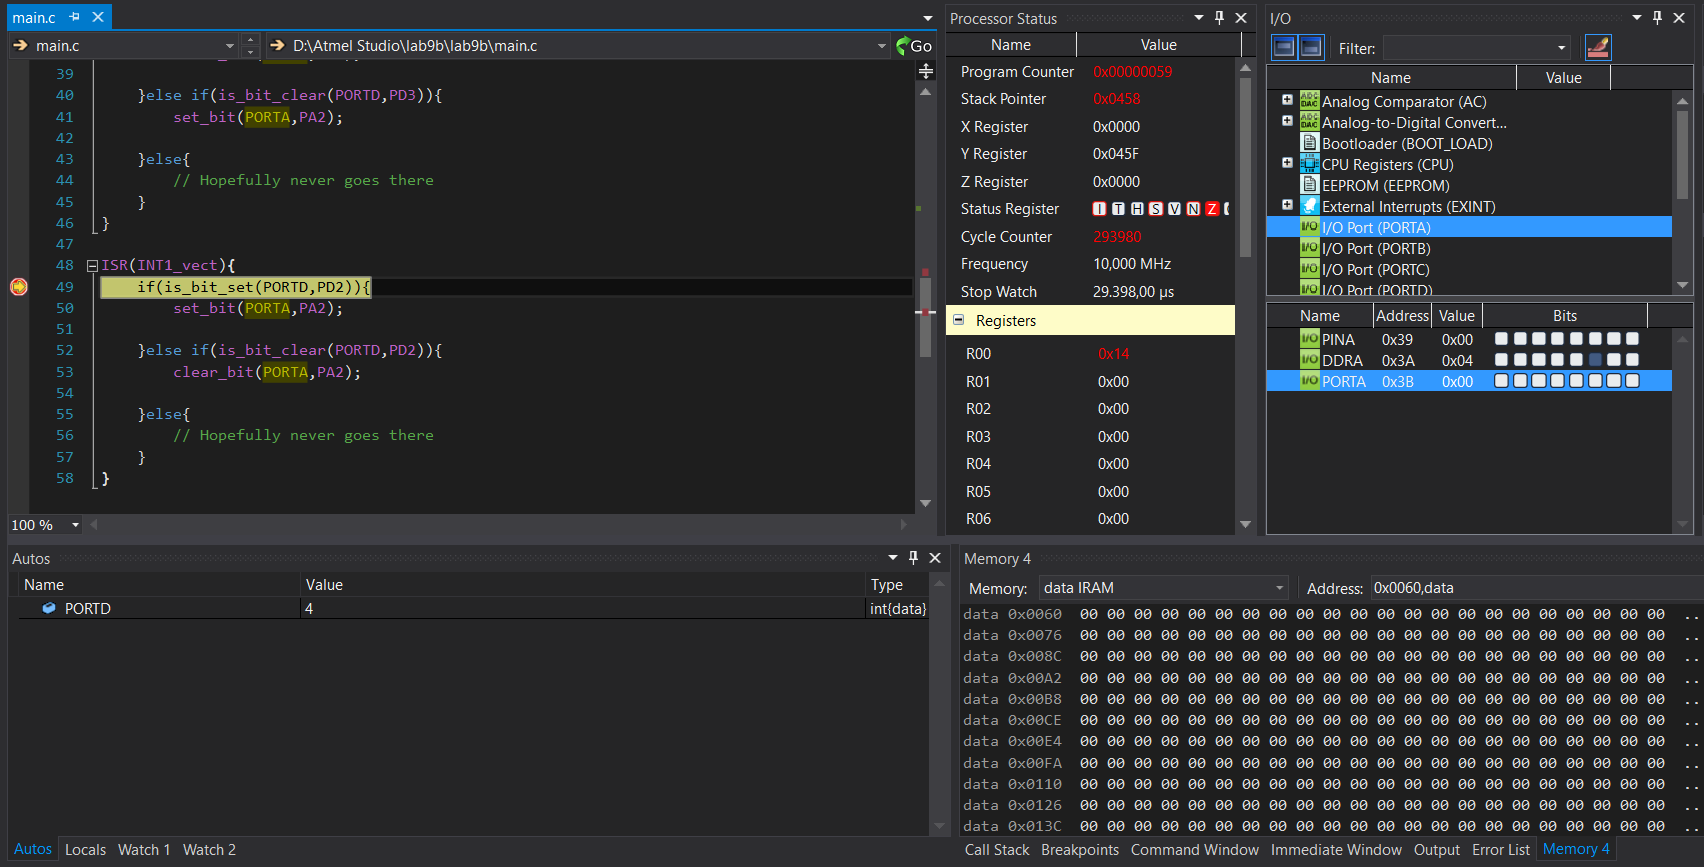
\includegraphics[height=3cm, width=\linewidth]{./results/lab9_sim_c_b.png}
		\end{subfigure}%
		~
		\begin{subfigure}[t]{0.5\textwidth}
			\centering
			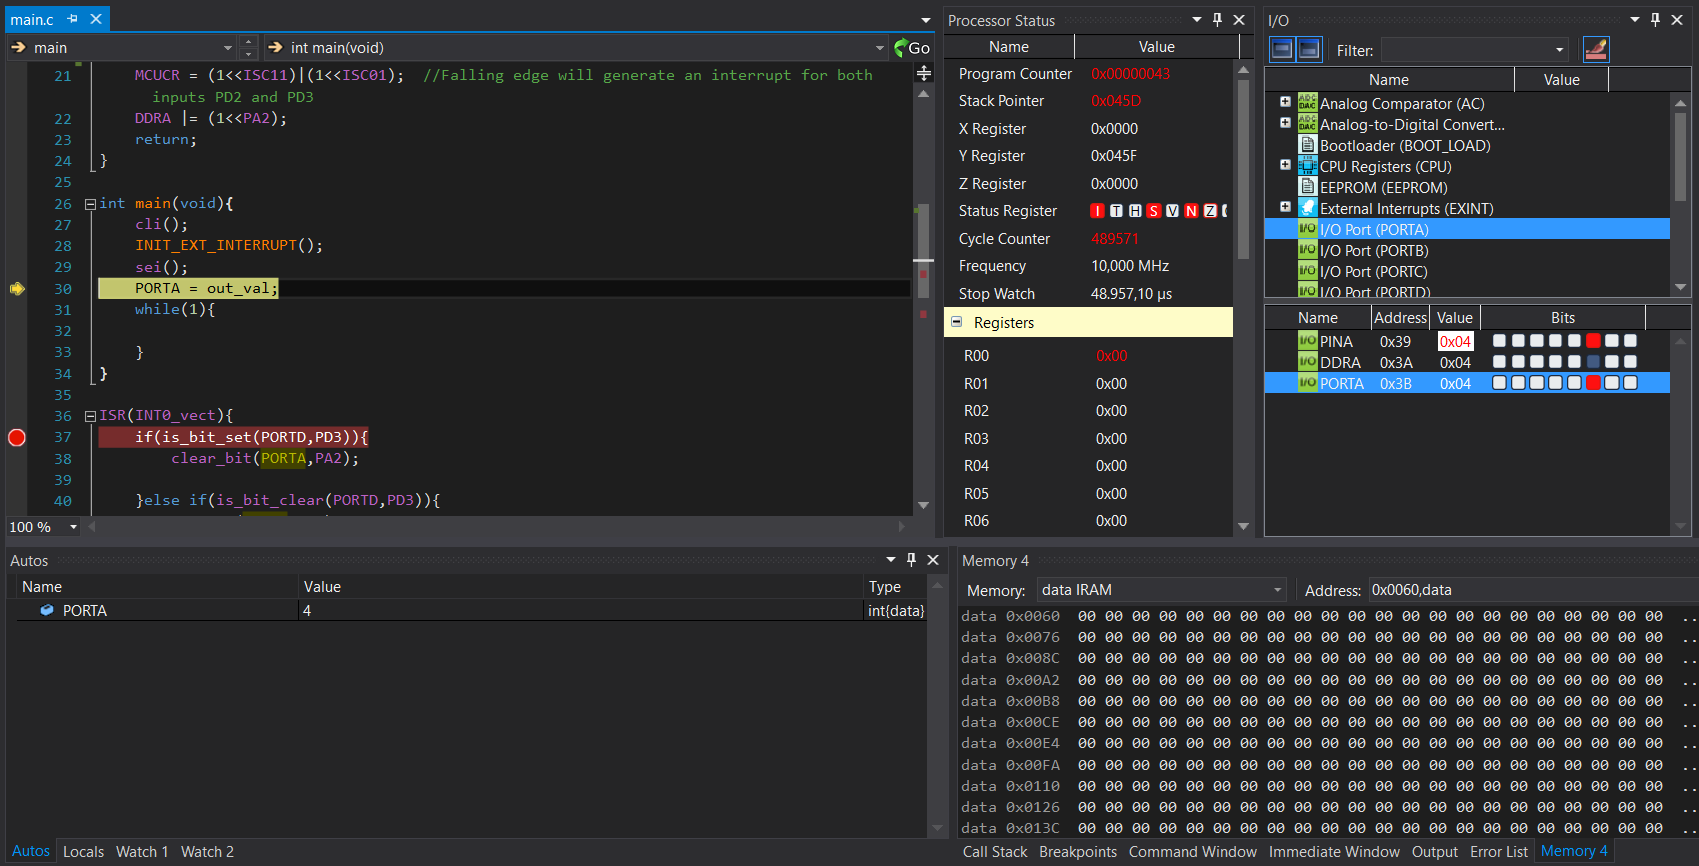
\includegraphics[height=3cm, width=\linewidth]{./results/lab9_sim_d_b.png}
		\end{subfigure}
		\caption{Results from Αtmel Studio 7 - Change from "1" to "0"}
	\end{figure}
\end{document}
